\documentclass[]{book}
\usepackage{lmodern}
\usepackage{amssymb,amsmath}
\usepackage{ifxetex,ifluatex}
\usepackage{fixltx2e} % provides \textsubscript
\ifnum 0\ifxetex 1\fi\ifluatex 1\fi=0 % if pdftex
  \usepackage[T1]{fontenc}
  \usepackage[utf8]{inputenc}
\else % if luatex or xelatex
  \ifxetex
    \usepackage{mathspec}
  \else
    \usepackage{fontspec}
  \fi
  \defaultfontfeatures{Ligatures=TeX,Scale=MatchLowercase}
\fi
% use upquote if available, for straight quotes in verbatim environments
\IfFileExists{upquote.sty}{\usepackage{upquote}}{}
% use microtype if available
\IfFileExists{microtype.sty}{%
\usepackage{microtype}
\UseMicrotypeSet[protrusion]{basicmath} % disable protrusion for tt fonts
}{}
\usepackage[margin=1in]{geometry}
\usepackage{hyperref}
\hypersetup{unicode=true,
            pdftitle={Brain Signal Processing: Basics of EEG Analysis},
            pdfauthor={Palani Thanaraj K},
            pdfborder={0 0 0},
            breaklinks=true}
\urlstyle{same}  % don't use monospace font for urls
\usepackage{natbib}
\bibliographystyle{apalike}
\usepackage{color}
\usepackage{fancyvrb}
\newcommand{\VerbBar}{|}
\newcommand{\VERB}{\Verb[commandchars=\\\{\}]}
\DefineVerbatimEnvironment{Highlighting}{Verbatim}{commandchars=\\\{\}}
% Add ',fontsize=\small' for more characters per line
\usepackage{framed}
\definecolor{shadecolor}{RGB}{248,248,248}
\newenvironment{Shaded}{\begin{snugshade}}{\end{snugshade}}
\newcommand{\AlertTok}[1]{\textcolor[rgb]{0.94,0.16,0.16}{#1}}
\newcommand{\AnnotationTok}[1]{\textcolor[rgb]{0.56,0.35,0.01}{\textbf{\textit{#1}}}}
\newcommand{\AttributeTok}[1]{\textcolor[rgb]{0.77,0.63,0.00}{#1}}
\newcommand{\BaseNTok}[1]{\textcolor[rgb]{0.00,0.00,0.81}{#1}}
\newcommand{\BuiltInTok}[1]{#1}
\newcommand{\CharTok}[1]{\textcolor[rgb]{0.31,0.60,0.02}{#1}}
\newcommand{\CommentTok}[1]{\textcolor[rgb]{0.56,0.35,0.01}{\textit{#1}}}
\newcommand{\CommentVarTok}[1]{\textcolor[rgb]{0.56,0.35,0.01}{\textbf{\textit{#1}}}}
\newcommand{\ConstantTok}[1]{\textcolor[rgb]{0.00,0.00,0.00}{#1}}
\newcommand{\ControlFlowTok}[1]{\textcolor[rgb]{0.13,0.29,0.53}{\textbf{#1}}}
\newcommand{\DataTypeTok}[1]{\textcolor[rgb]{0.13,0.29,0.53}{#1}}
\newcommand{\DecValTok}[1]{\textcolor[rgb]{0.00,0.00,0.81}{#1}}
\newcommand{\DocumentationTok}[1]{\textcolor[rgb]{0.56,0.35,0.01}{\textbf{\textit{#1}}}}
\newcommand{\ErrorTok}[1]{\textcolor[rgb]{0.64,0.00,0.00}{\textbf{#1}}}
\newcommand{\ExtensionTok}[1]{#1}
\newcommand{\FloatTok}[1]{\textcolor[rgb]{0.00,0.00,0.81}{#1}}
\newcommand{\FunctionTok}[1]{\textcolor[rgb]{0.00,0.00,0.00}{#1}}
\newcommand{\ImportTok}[1]{#1}
\newcommand{\InformationTok}[1]{\textcolor[rgb]{0.56,0.35,0.01}{\textbf{\textit{#1}}}}
\newcommand{\KeywordTok}[1]{\textcolor[rgb]{0.13,0.29,0.53}{\textbf{#1}}}
\newcommand{\NormalTok}[1]{#1}
\newcommand{\OperatorTok}[1]{\textcolor[rgb]{0.81,0.36,0.00}{\textbf{#1}}}
\newcommand{\OtherTok}[1]{\textcolor[rgb]{0.56,0.35,0.01}{#1}}
\newcommand{\PreprocessorTok}[1]{\textcolor[rgb]{0.56,0.35,0.01}{\textit{#1}}}
\newcommand{\RegionMarkerTok}[1]{#1}
\newcommand{\SpecialCharTok}[1]{\textcolor[rgb]{0.00,0.00,0.00}{#1}}
\newcommand{\SpecialStringTok}[1]{\textcolor[rgb]{0.31,0.60,0.02}{#1}}
\newcommand{\StringTok}[1]{\textcolor[rgb]{0.31,0.60,0.02}{#1}}
\newcommand{\VariableTok}[1]{\textcolor[rgb]{0.00,0.00,0.00}{#1}}
\newcommand{\VerbatimStringTok}[1]{\textcolor[rgb]{0.31,0.60,0.02}{#1}}
\newcommand{\WarningTok}[1]{\textcolor[rgb]{0.56,0.35,0.01}{\textbf{\textit{#1}}}}
\usepackage{longtable,booktabs}
\usepackage{graphicx,grffile}
\makeatletter
\def\maxwidth{\ifdim\Gin@nat@width>\linewidth\linewidth\else\Gin@nat@width\fi}
\def\maxheight{\ifdim\Gin@nat@height>\textheight\textheight\else\Gin@nat@height\fi}
\makeatother
% Scale images if necessary, so that they will not overflow the page
% margins by default, and it is still possible to overwrite the defaults
% using explicit options in \includegraphics[width, height, ...]{}
\setkeys{Gin}{width=\maxwidth,height=\maxheight,keepaspectratio}
\IfFileExists{parskip.sty}{%
\usepackage{parskip}
}{% else
\setlength{\parindent}{0pt}
\setlength{\parskip}{6pt plus 2pt minus 1pt}
}
\setlength{\emergencystretch}{3em}  % prevent overfull lines
\providecommand{\tightlist}{%
  \setlength{\itemsep}{0pt}\setlength{\parskip}{0pt}}
\setcounter{secnumdepth}{5}
% Redefines (sub)paragraphs to behave more like sections
\ifx\paragraph\undefined\else
\let\oldparagraph\paragraph
\renewcommand{\paragraph}[1]{\oldparagraph{#1}\mbox{}}
\fi
\ifx\subparagraph\undefined\else
\let\oldsubparagraph\subparagraph
\renewcommand{\subparagraph}[1]{\oldsubparagraph{#1}\mbox{}}
\fi

%%% Use protect on footnotes to avoid problems with footnotes in titles
\let\rmarkdownfootnote\footnote%
\def\footnote{\protect\rmarkdownfootnote}

%%% Change title format to be more compact
\usepackage{titling}

% Create subtitle command for use in maketitle
\providecommand{\subtitle}[1]{
  \posttitle{
    \begin{center}\large#1\end{center}
    }
}

\setlength{\droptitle}{-2em}

  \title{Brain Signal Processing: Basics of EEG Analysis}
    \pretitle{\vspace{\droptitle}\centering\huge}
  \posttitle{\par}
    \author{Palani Thanaraj K}
    \preauthor{\centering\large\emph}
  \postauthor{\par}
      \predate{\centering\large\emph}
  \postdate{\par}
    \date{2020-03-30}

\usepackage{booktabs}

\begin{document}
\maketitle

{
\setcounter{tocdepth}{1}
\tableofcontents
}
\hypertarget{prerequisites}{%
\chapter*{Prerequisites}\label{prerequisites}}
\addcontentsline{toc}{chapter}{Prerequisites}

This tutorial provides basics of EEG analysis with minimal coding using Python. So not much of technical knowledge is required for going through this tutorial. As and when some jargon is encountered it is provided with required information. Feel free to go through this tutorial.

\hypertarget{intro}{%
\chapter{Introduction}\label{intro}}

EEG is the recording of electrical signals obtained from the scalp region of the human head. It is because of the activation of the pyramidal neurons in the cerebral cortex region of the brain (i.e outer layer of the brain).

\hypertarget{how-eeg-is-used-in-clinical-setting}{%
\section{How EEG is used in clinical setting}\label{how-eeg-is-used-in-clinical-setting}}

EEG represents the functional operation of the brain. The EEG signal is also referred to as Brain Waves that are named based on the frequency component in the signal. They are Delta, Theta, Alpha, Beta, and Gamma brain waves. Their frequency component falls in the range of 1-3,3-7,7-13,13-30 and \textgreater30 Hz respectively. EEG is used in the management of brain disorders such as Epilepsy, Schizophrenia (SZ) and Alzhemier's disease. In this tutorial, we will discuss about some aspects of Schizophrenia disease and its assessment using EEG signal.

\hypertarget{what-is-schizophrenia-condition}{%
\chapter{What is Schizophrenia condition?}\label{what-is-schizophrenia-condition}}

Schizophrenia is a detrimental condition of the brain which leads to reduction in the cognitive awareness. The patients affected by this disease try to have impairment in assessing day-to-day activities. EEG is an important modality that can detect the SZ occurrence in an individual. The EEG signal shows low randomness compared to a healthy person. Here we will take few EEG signal of normal and SZ patients and analyse them.

\hypertarget{dataset}{%
\section{Dataset}\label{dataset}}

The SZ dataset which we are going to analyse here is from ``EEG in schizophrenia (RepOD)'' from the seminal works of \citep{eeg-in-schizophrenia}. The dataset comprised 14 patients with paranoid schizophrenia and 14 healthy controls. Data were acquired with the sampling frequency of 250 Hz using the standard 10-20 EEG montage with 19 EEG channels: Fp1, Fp2, F7, F3, Fz, F4, F8, T3, C3, Cz, C4, T4, T5, P3, Pz, P4, T6, O1, O2. The reference electrode was placed between electrodes Fz and Cz. ~

\hypertarget{eeg-data-import-analysis}{%
\chapter{EEG data import \& Analysis}\label{eeg-data-import-analysis}}

The EEG data is available in the '*.edf' file extension. We have to download the EEG files and place in the working directory of the Python program such as Jupyter notebook or Spyder. Then we will be using the MNE Python library for the processing of the EEG signal. The following section provides the code block for import the necessary library files for EEG analysis.

\hypertarget{mne-library-for-eeg-analysis}{%
\section{MNE Library for EEG Analysis}\label{mne-library-for-eeg-analysis}}

\begin{Shaded}
\begin{Highlighting}[]
\ImportTok{import}\NormalTok{ mne }\CommentTok{# MNE library for EEG analysis}
\ImportTok{import}\NormalTok{ matplotlib.pyplot }\ImportTok{as}\NormalTok{ plt }\CommentTok{# Plotting library}

\NormalTok{plt.style.use(}\StringTok{'seaborn-bright'}\NormalTok{) }\CommentTok{# Plot Style}
\NormalTok{plt.rcParams[}\StringTok{'figure.dpi'}\NormalTok{] }\OperatorTok{=} \DecValTok{300} \CommentTok{# DPI setting}
\NormalTok{plt.rcParams[}\StringTok{'figure.figsize'}\NormalTok{] }\OperatorTok{=}\NormalTok{ (}\DecValTok{8}\NormalTok{, }\DecValTok{6}\NormalTok{)}
\end{Highlighting}
\end{Shaded}

\hypertarget{data-import}{%
\section{Data Import}\label{data-import}}

This code chunk explains how to import the EEG file into the Python workspace by the command \texttt{mne.io.read\_raw\_edf}. Moreover, it also shows the file info of the EEG file imported into the workspace.

\begin{Shaded}
\begin{Highlighting}[]
\CommentTok{# Data import}
\NormalTok{raw_h }\OperatorTok{=}\NormalTok{ mne.io.read_raw_edf(}\StringTok{"h01.edf"}\NormalTok{, preload}\OperatorTok{=}\VariableTok{True}\NormalTok{)}\CommentTok{# Import data file into workspace}
\CommentTok{# h01 specifies the EEG record of healthy control-1}
\end{Highlighting}
\end{Shaded}

\begin{verbatim}
## Extracting EDF parameters from C:\Users\RajuPC\Documents\MyR\MyGitbook\EEG\EEG_analysis\h01.edf...
## EDF file detected
## Setting channel info structure...
## Creating raw.info structure...
## Reading 0 ... 231249  =      0.000 ...   924.996 secs...
\end{verbatim}

\begin{Shaded}
\begin{Highlighting}[]
\NormalTok{raw_s }\OperatorTok{=}\NormalTok{ mne.io.read_raw_edf(}\StringTok{"s01.edf"}\NormalTok{, preload}\OperatorTok{=}\VariableTok{True}\NormalTok{)}\CommentTok{# Import data file into workspace}
\CommentTok{# s01 specifies the EEG record of SZ patient-1}

\CommentTok{# Give the sample rate}
\end{Highlighting}
\end{Shaded}

\begin{verbatim}
## Extracting EDF parameters from C:\Users\RajuPC\Documents\MyR\MyGitbook\EEG\EEG_analysis\s01.edf...
## EDF file detected
## Setting channel info structure...
## Creating raw.info structure...
## Reading 0 ... 211249  =      0.000 ...   844.996 secs...
\end{verbatim}

\begin{Shaded}
\begin{Highlighting}[]
\BuiltInTok{print}\NormalTok{(}\StringTok{'sample rate:'}\NormalTok{, raw_h.info[}\StringTok{'sfreq'}\NormalTok{], }\StringTok{'Hz'}\NormalTok{)}
\CommentTok{# Give the size of the data matrix}
\end{Highlighting}
\end{Shaded}

\begin{verbatim}
## sample rate: 250.0 Hz
\end{verbatim}

\begin{Shaded}
\begin{Highlighting}[]
\BuiltInTok{print}\NormalTok{(}\StringTok{'Data matrix size : }\SpecialCharTok{%s}\StringTok{ channels x }\SpecialCharTok\NormalTok{ (raw_h.info[}\StringTok{'nchan'}\NormalTok{], }\BuiltInTok{len}\NormalTok{(raw_h.times)))}
\end{Highlighting}
\end{Shaded}

\begin{verbatim}
## Data matrix size : 19 channels x 231250 samples
\end{verbatim}

\begin{Shaded}
\begin{Highlighting}[]
\BuiltInTok{print}\NormalTok{(}\StringTok{'Channel names:'}\NormalTok{, raw_h.info[}\StringTok{'ch_names'}\NormalTok{])}
\end{Highlighting}
\end{Shaded}

\begin{verbatim}
## Channel names: ['Fp2', 'F8', 'T4', 'T6', 'O2', 'Fp1', 'F7', 'T3', 'T5', 'O1', 'F4', 'C4', 'P4', 'F3', 'C3', 'P3', 'Fz', 'Cz', 'Pz']
\end{verbatim}

\hypertarget{time-series-plot-of-the-eeg-signal}{%
\section{Time series plot of the EEG signal}\label{time-series-plot-of-the-eeg-signal}}

This code plots the raw EEG signal using the available function \texttt{plot}.
Healthy Individual

\begin{Shaded}
\begin{Highlighting}[]
\CommentTok{# Plotting the raw EEG signal}
\NormalTok{raw_h.plot(start}\OperatorTok{=}\DecValTok{300}\NormalTok{,duration}\OperatorTok{=}\DecValTok{2}\NormalTok{, block}\OperatorTok{=}\VariableTok{True}\NormalTok{, show}\OperatorTok{=}\VariableTok{False}\NormalTok{, color}\OperatorTok{=}\StringTok{'green'}\NormalTok{)}
\end{Highlighting}
\end{Shaded}

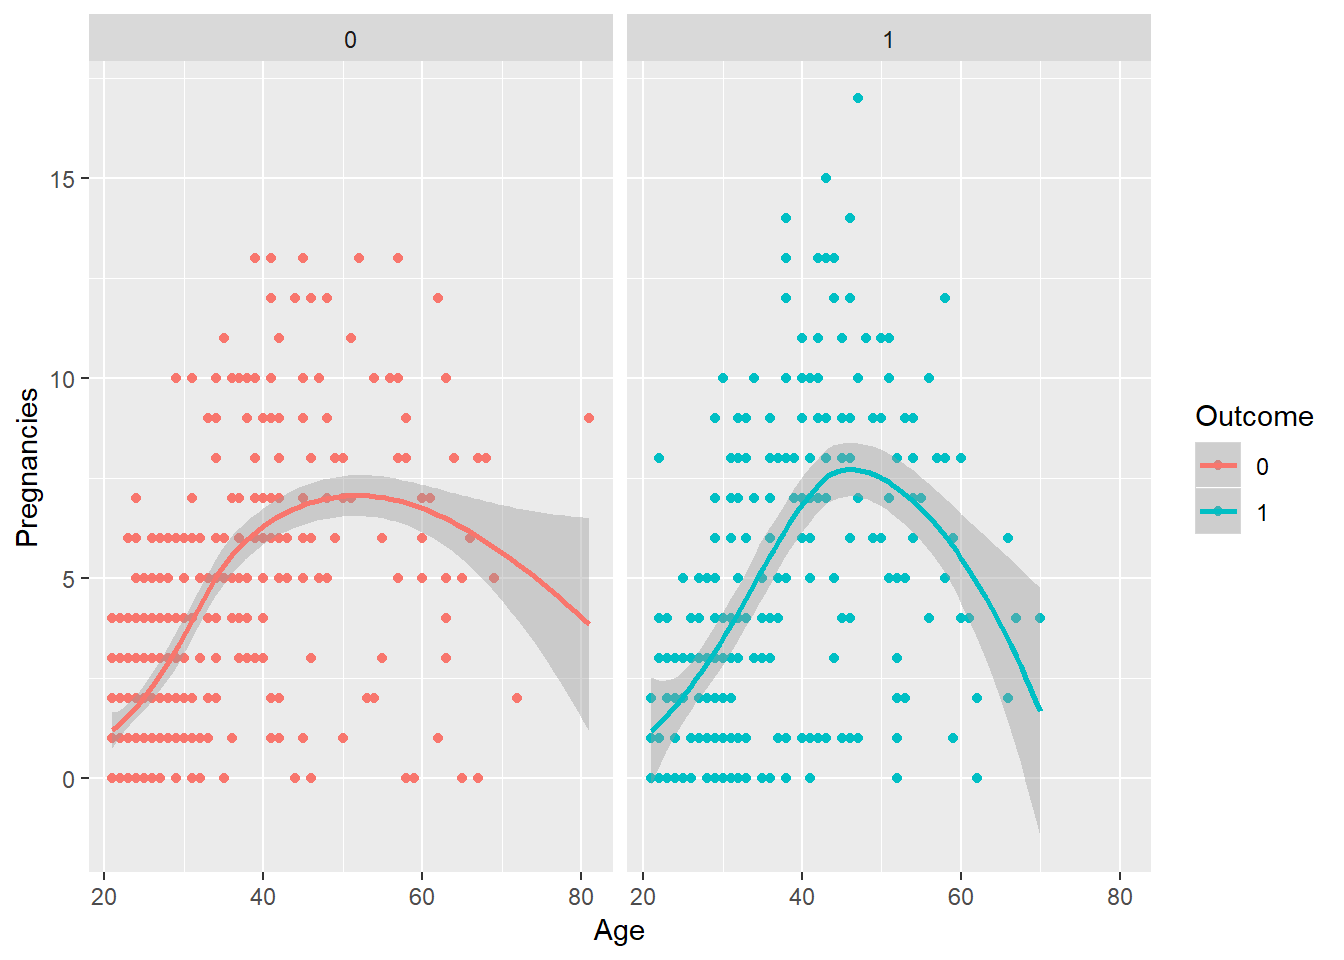
\includegraphics{EEG_analysis_files/figure-latex/unnamed-chunk-4-1.pdf}

SZ Patient

\begin{Shaded}
\begin{Highlighting}[]
\CommentTok{# Plotting the raw EEG signal}
\NormalTok{raw_s.plot(start}\OperatorTok{=}\DecValTok{300}\NormalTok{,duration}\OperatorTok{=}\DecValTok{2}\NormalTok{, block}\OperatorTok{=}\VariableTok{True}\NormalTok{, show}\OperatorTok{=}\VariableTok{False}\NormalTok{, color}\OperatorTok{=}\StringTok{'red'}\NormalTok{)}
\end{Highlighting}
\end{Shaded}

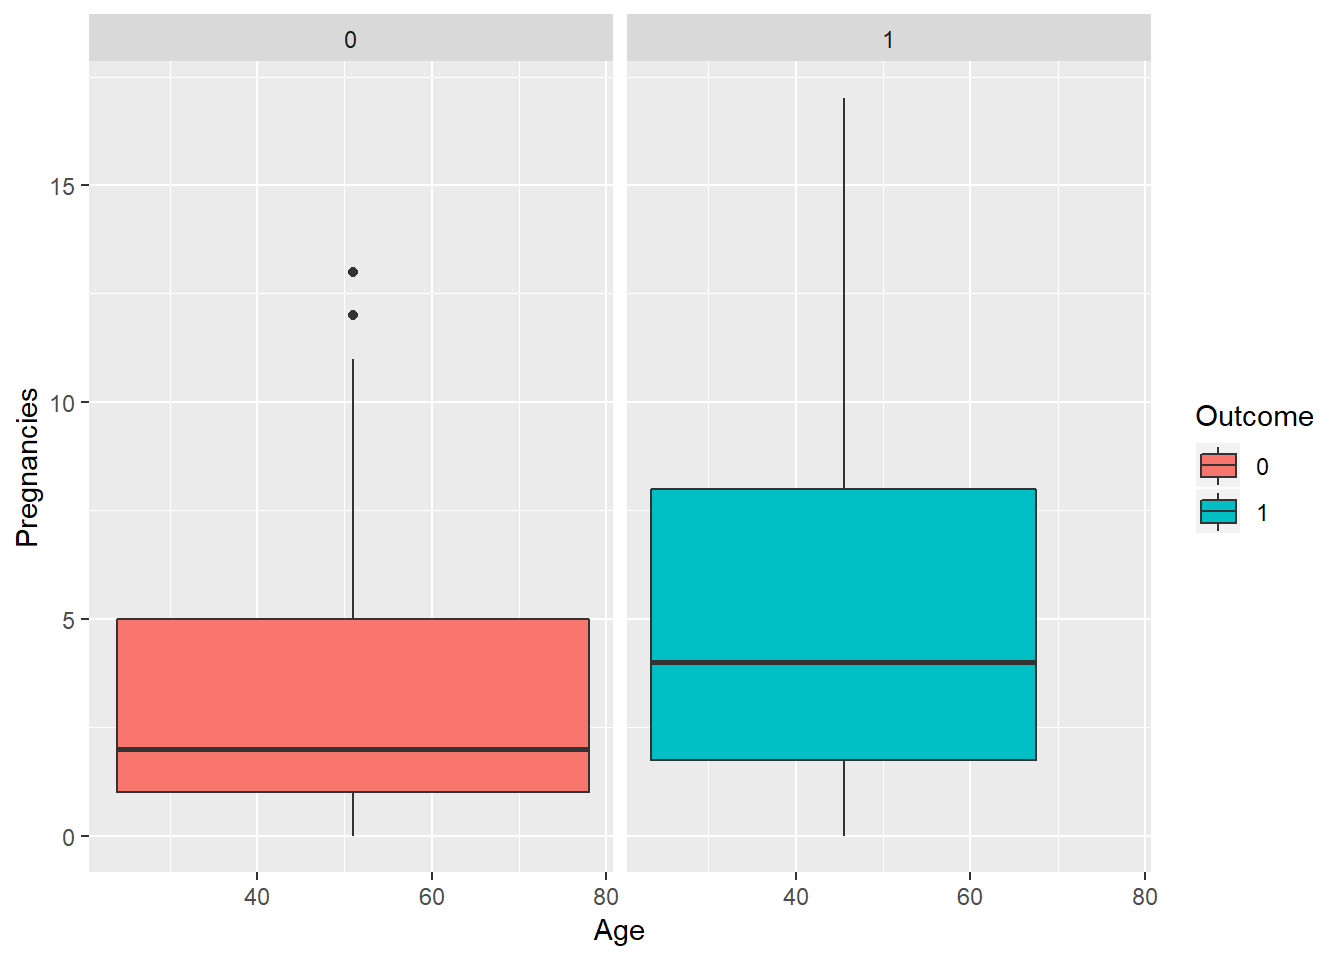
\includegraphics{EEG_analysis_files/figure-latex/unnamed-chunk-5-1.pdf}

\hypertarget{bandpass-filtering-of-the-eeg-signal}{%
\section{Bandpass filtering of the EEG signal}\label{bandpass-filtering-of-the-eeg-signal}}

This code applies a FIR filter based on windowing technique to design a bandpass filter with lower cut-off frequency at 0.5Hz and upper cut-off frequency at 100Hz.
Healthy Control

\begin{Shaded}
\begin{Highlighting}[]
\NormalTok{xfil_h}\OperatorTok{=}\NormalTok{raw_h.}\BuiltInTok{filter}\NormalTok{(}\FloatTok{0.5}\NormalTok{, }\FloatTok{100.}\NormalTok{, fir_design}\OperatorTok{=}\StringTok{'firwin'}\NormalTok{)}\CommentTok{#Bandpass filtering}
\end{Highlighting}
\end{Shaded}

\begin{verbatim}
## Filtering raw data in 1 contiguous segment
## Setting up band-pass filter from 0.5 - 1e+02 Hz
## 
## FIR filter parameters
## ---------------------
## Designing a one-pass, zero-phase, non-causal bandpass filter:
## - Windowed time-domain design (firwin) method
## - Hamming window with 0.0194 passband ripple and 53 dB stopband attenuation
## - Lower passband edge: 0.50
## - Lower transition bandwidth: 0.50 Hz (-6 dB cutoff frequency: 0.25 Hz)
## - Upper passband edge: 100.00 Hz
## - Upper transition bandwidth: 25.00 Hz (-6 dB cutoff frequency: 112.50 Hz)
## - Filter length: 1651 samples (6.604 sec)
\end{verbatim}

\begin{Shaded}
\begin{Highlighting}[]
\NormalTok{xfil_h.plot(start}\OperatorTok{=}\DecValTok{300}\NormalTok{, duration}\OperatorTok{=}\DecValTok{2}\NormalTok{, bgcolor}\OperatorTok{=}\StringTok{'w'}\NormalTok{,show}\OperatorTok{=}\VariableTok{False}\NormalTok{, events}\OperatorTok{=}\VariableTok{None}\NormalTok{,proj}\OperatorTok{=}\VariableTok{False}\NormalTok{,color}\OperatorTok{=}\StringTok{'green'}\NormalTok{)}\CommentTok{#plotting of the filtered signal}
\end{Highlighting}
\end{Shaded}

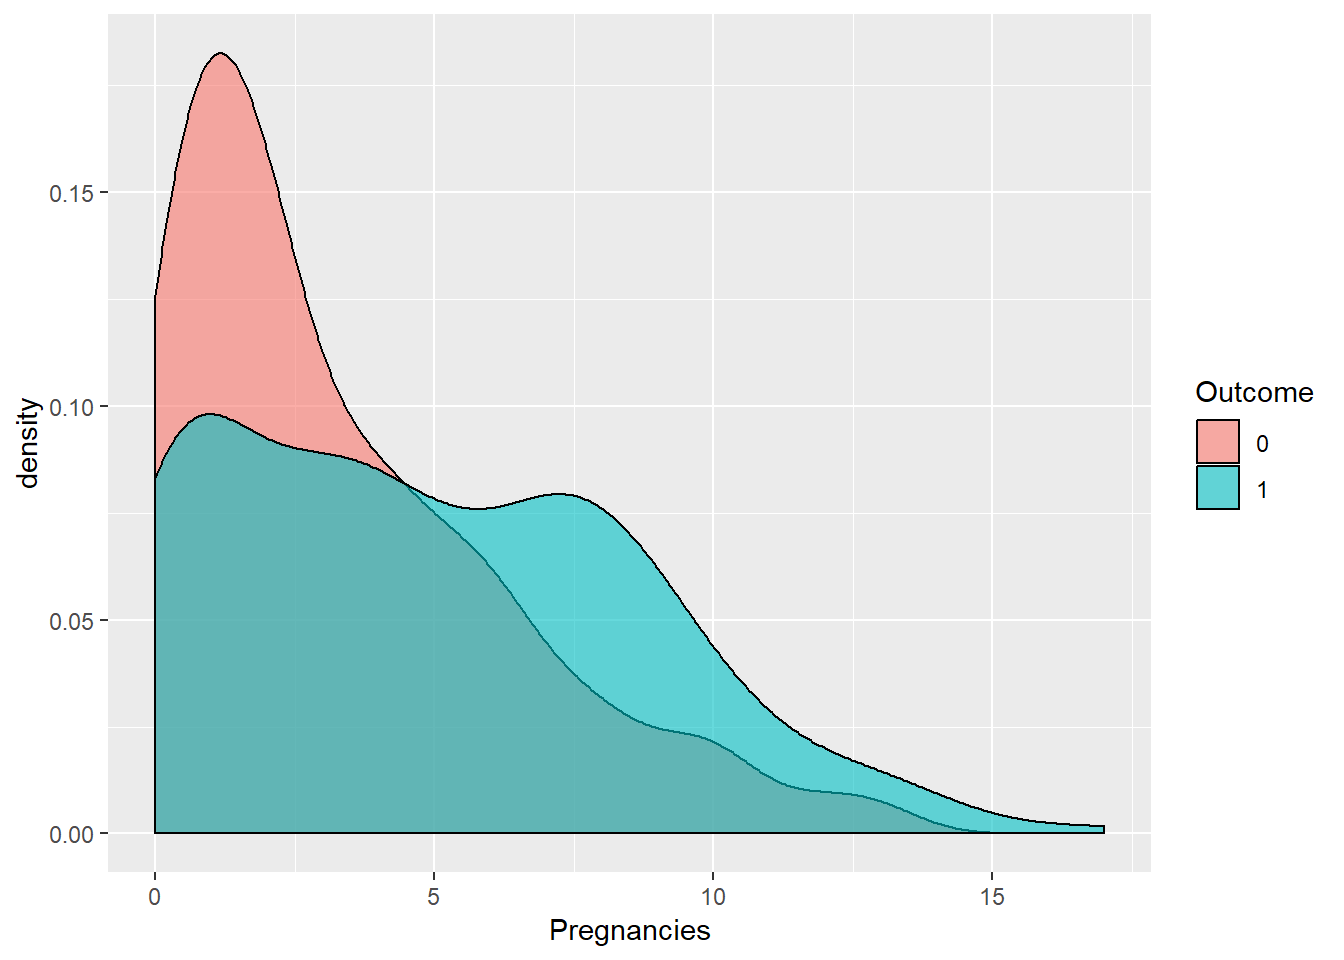
\includegraphics{EEG_analysis_files/figure-latex/unnamed-chunk-6-1.pdf}

SZ patient

\begin{Shaded}
\begin{Highlighting}[]
\NormalTok{xfil_s}\OperatorTok{=}\NormalTok{raw_s.}\BuiltInTok{filter}\NormalTok{(}\FloatTok{0.5}\NormalTok{, }\FloatTok{100.}\NormalTok{, fir_design}\OperatorTok{=}\StringTok{'firwin'}\NormalTok{)}\CommentTok{#Bandpass filtering}
\end{Highlighting}
\end{Shaded}

\begin{verbatim}
## Filtering raw data in 1 contiguous segment
## Setting up band-pass filter from 0.5 - 1e+02 Hz
## 
## FIR filter parameters
## ---------------------
## Designing a one-pass, zero-phase, non-causal bandpass filter:
## - Windowed time-domain design (firwin) method
## - Hamming window with 0.0194 passband ripple and 53 dB stopband attenuation
## - Lower passband edge: 0.50
## - Lower transition bandwidth: 0.50 Hz (-6 dB cutoff frequency: 0.25 Hz)
## - Upper passband edge: 100.00 Hz
## - Upper transition bandwidth: 25.00 Hz (-6 dB cutoff frequency: 112.50 Hz)
## - Filter length: 1651 samples (6.604 sec)
\end{verbatim}

\begin{Shaded}
\begin{Highlighting}[]
\NormalTok{xfil_s.plot(start}\OperatorTok{=}\DecValTok{300}\NormalTok{, duration}\OperatorTok{=}\DecValTok{2}\NormalTok{, bgcolor}\OperatorTok{=}\StringTok{'w'}\NormalTok{,show}\OperatorTok{=}\VariableTok{False}\NormalTok{, events}\OperatorTok{=}\VariableTok{None}\NormalTok{,proj}\OperatorTok{=}\VariableTok{False}\NormalTok{,color}\OperatorTok{=}\StringTok{'red'}\NormalTok{)}\CommentTok{#plotting of the filtered signal}
\end{Highlighting}
\end{Shaded}

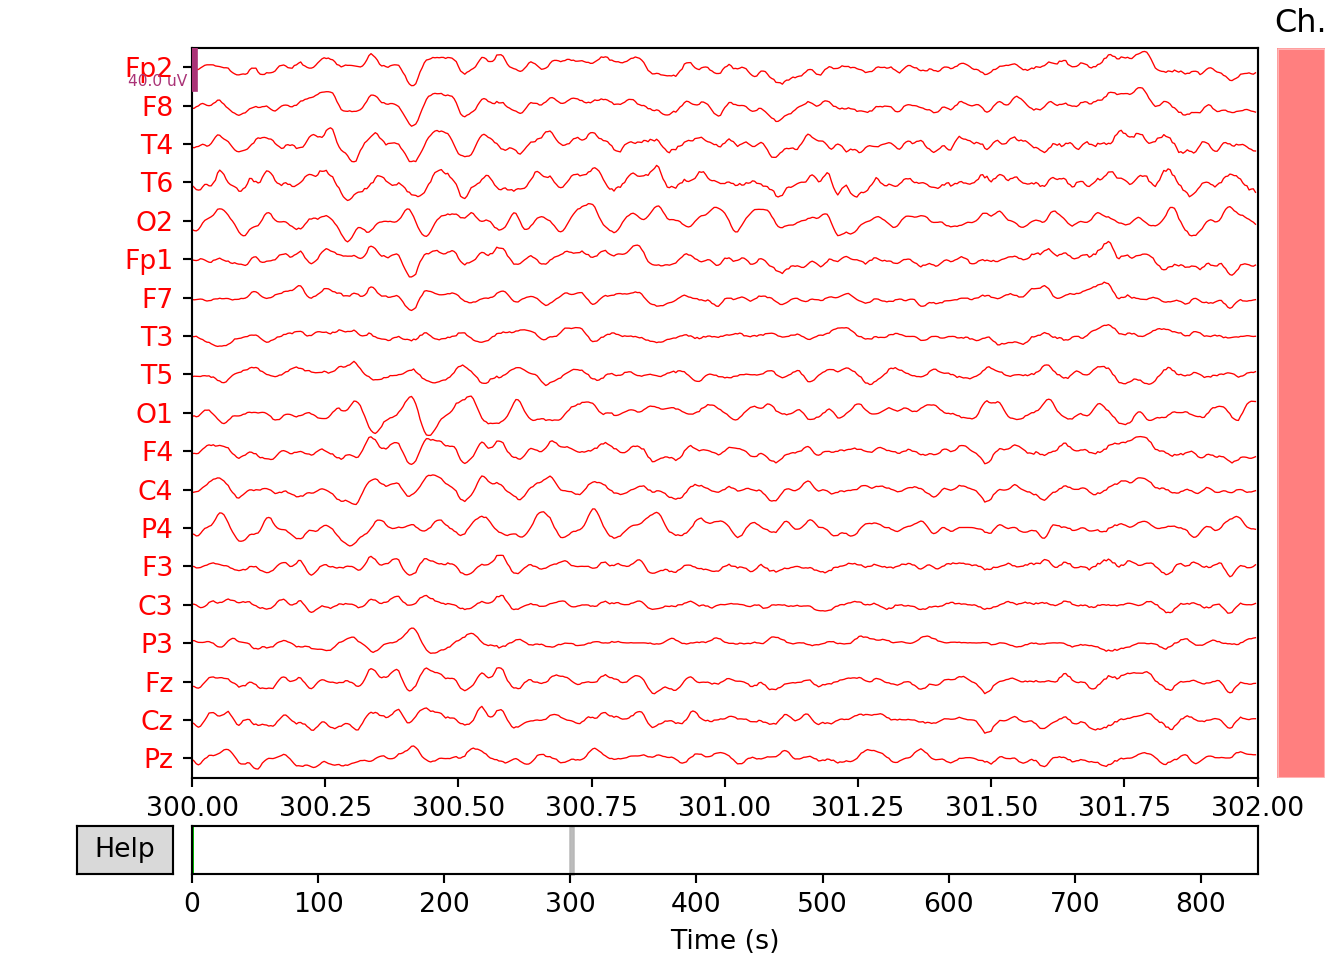
\includegraphics{EEG_analysis_files/figure-latex/unnamed-chunk-7-1.pdf}

\hypertarget{the-power-spectral-density-psdfunction-of-the-eeg-signal}{%
\section{The power spectral density (PSD)function of the EEG signal}\label{the-power-spectral-density-psdfunction-of-the-eeg-signal}}

This code performs the Power Spectral Density (PSD) function of the Filtered EEG signal.
Healthy Control

\begin{Shaded}
\begin{Highlighting}[]
\NormalTok{xfil_h.plot_psd(area_mode}\OperatorTok{=}\StringTok{'range'}\NormalTok{, tmax}\OperatorTok{=}\FloatTok{10.0}\NormalTok{, show}\OperatorTok{=}\VariableTok{False}\NormalTok{, average}\OperatorTok{=}\VariableTok{True}\NormalTok{, color}\OperatorTok{=}\StringTok{'green'}\NormalTok{)}
\end{Highlighting}
\end{Shaded}

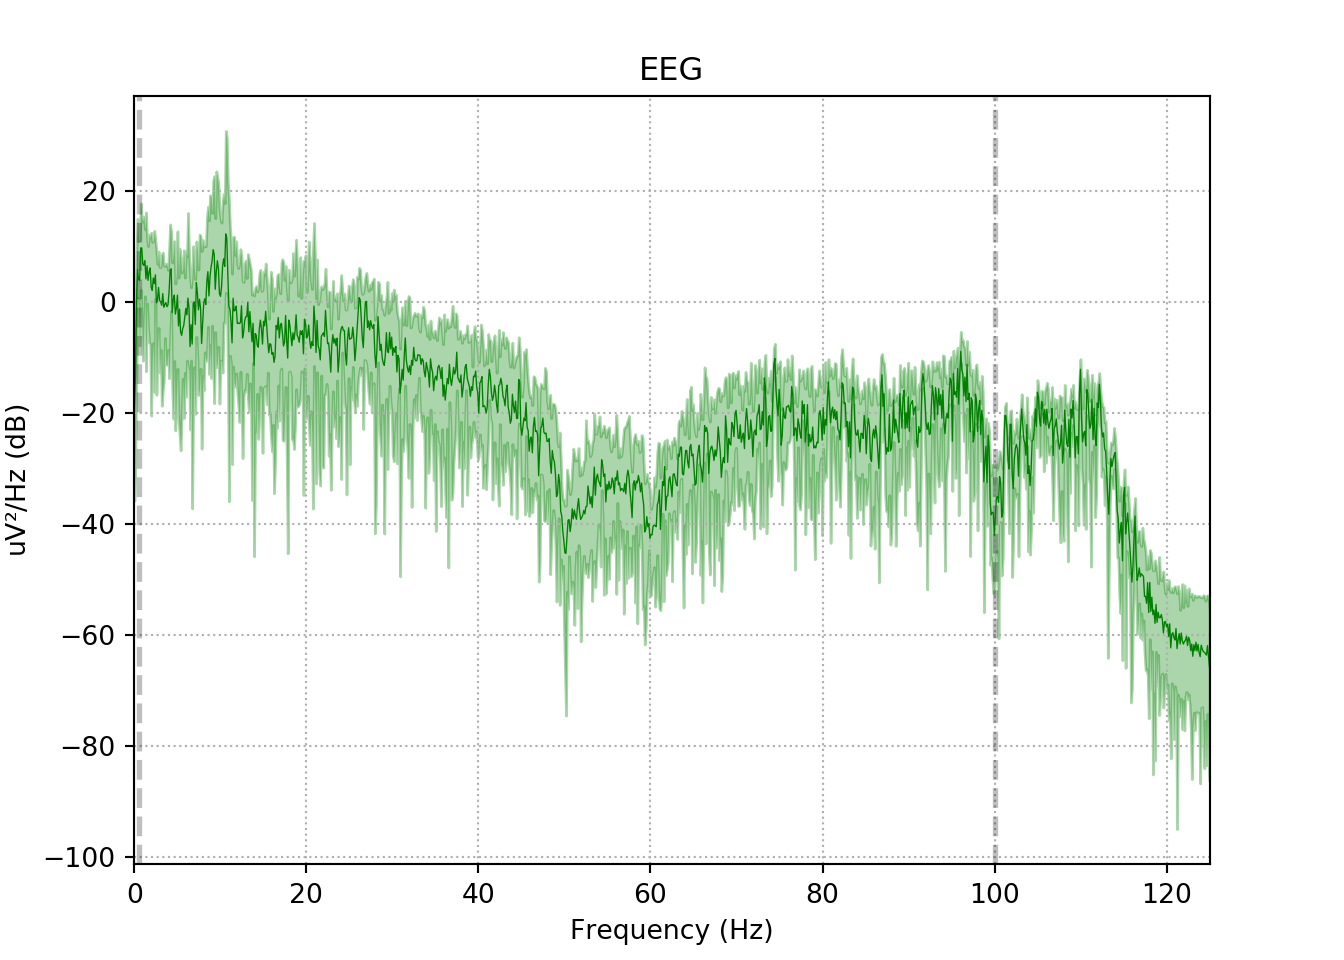
\includegraphics{EEG_analysis_files/figure-latex/unnamed-chunk-8-1.pdf}

SZ Patient

\begin{Shaded}
\begin{Highlighting}[]
\NormalTok{xfil_s.plot_psd(area_mode}\OperatorTok{=}\StringTok{'range'}\NormalTok{, tmax}\OperatorTok{=}\FloatTok{10.0}\NormalTok{, show}\OperatorTok{=}\VariableTok{False}\NormalTok{, average}\OperatorTok{=}\VariableTok{True}\NormalTok{, color}\OperatorTok{=}\StringTok{'red'}\NormalTok{)}
\end{Highlighting}
\end{Shaded}

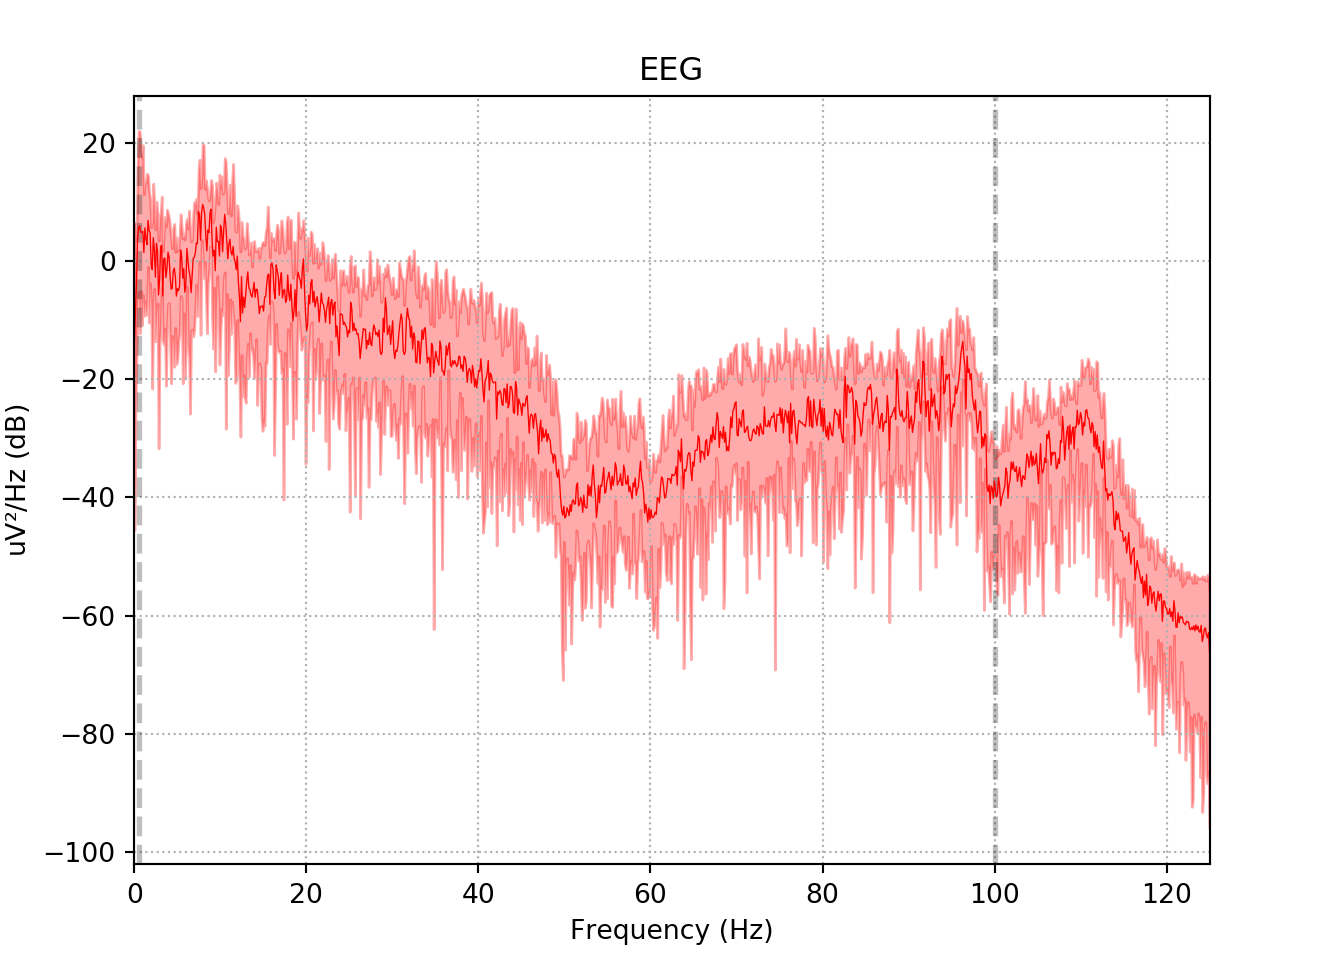
\includegraphics{EEG_analysis_files/figure-latex/unnamed-chunk-9-1.pdf}

\hypertarget{more-links}{%
\section{More Links}\label{more-links}}

More information related to applications of EEG in brain disorders can be found in the following articles:

\begin{itemize}
\tightlist
\item
  \citep{T.Krishnan2016}
\item
  \citep{Thanaraj2014}
\item
  \citep{Krishnan2017}
\item
  \citep{Krishnan2017a}
\item
  \citep{Thanaraj2017}
\item
  \citep{Abhinaya2016}
\item
  \citep{Johannesen2016}
\item
  \citep{Gotz2017}
\item
  \citep{Thilakvathi2017}
\item
  \citep{Olejarczyk2017}
\end{itemize}

\bibliography{book.bib}


\end{document}
